\subsection{Gesamtablauf der auftragsbasierten Auslagerung}

Zu Beginn der Implementierung der Auftragssteuerung wurde das vorhandene System betrachtet.\\
Der Auslagerprozess wurde bereits in der Dokumentation der vorherigen Studienarbeit beschrieben und wird deshalb an dieser Stelle nicht erneut im Detail erläutert.\\

\subsubsection{Anbindung der Materialdaten}

Im bestehenden Konzept sind die verschiedenen Materialien innerhalb der SPS in Form einer Textliste hinterlegt. Diese Art der Datenhaltung ist jedoch nur eingeschränkt geeignet, da sie eine Erweiterung sowie eine flexible Verarbeitung der Daten erschwert.\\

Aus diesem Grund wurde eine externe Datenstruktur eingeführt, welche auf einem separaten Rechner gespeichert wird. Diese kann beispielsweise in Form einer \textbf{CSV-Datei} realisiert werden und enthält die relevanten Materialinformationen.\\

\begin{figure}[H]
	\centering
	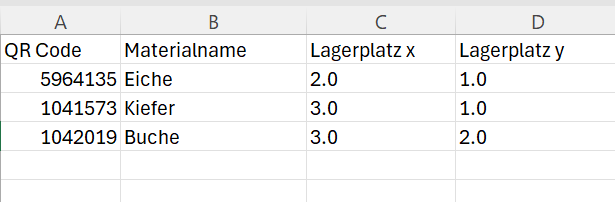
\includegraphics[width=0.5\textwidth]{Screenshots/Auftragsbasierte Auslagerung/CSV_Datei.png}
	\caption{Beispielhafte Struktur der Materialdaten}
	\label{fig:csv}
\end{figure}

In Abbildung \ref{fig:csv} ist ein exemplarischer Aufbau der verwendeten Materialdaten dargestellt. Diese umfasst unter anderem:
\begin{itemize}
	\item Lagerplatz
	\item QR Code (Artikelnummer)
	\item Artikelname
\end{itemize}

Durch die Auslagerung der Daten in eine externe Struktur wird eine deutlich höhere Flexibilität erreicht. Neue Materialien können ohne Anpassung der SPS ergänzt werden, wodurch das System leichter erweiterbar ist.\\

\subsubsection{Aufbau der Programmanwendung}

Zur Verarbeitung der Materialdaten wurde eine eigene Programmanwendung entwickelt. Diese stellt das zentrale Bindeglied zwischen der Datenspeicherung und der SPS dar.\\

Der grundlegende Aufbau der Anwendung gliedert sich in zwei Funktionsbereiche:
\begin{itemize}
	\item Verarbeitungsebene zur Einlesung und Aufbereitung der Materialdaten
	\item Auftragsebene zur Kommunikation mit der SPS
\end{itemize}

Innerhalb der Verarbeitungsebene werden die Materialdaten eingelesen und in eine geeignete Struktur überführt. Hierbei werden die relevanten Informationen extrahiert und für die weitere Nutzung vorbereitet.\\

Die Auftragsebene baut auf diesen aufbereiteten Daten auf und übernimmt die Kommunikation mit der \textbf{SPS}. In diesem Schritt werden die notwendigen Steuerinformationen generiert und an die Steuerung übertragen, wodurch der Auslagerprozess ausgelöst wird.
\subsubsection{Verarbeitung der Materialdaten}

Die Verarbeitung der Materialdaten stellt einen zentralen Bestandteil der entwickelten Programmanwendung dar. Ziel ist es, die eingelesenen Daten aus der externen Datenstruktur auszuwerten und für die weitere Verwendung im System bereitzustellen.\\
\begin{figure}[H]
	\centering
	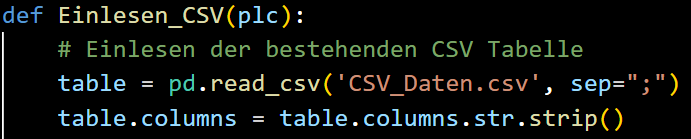
\includegraphics[width=0.6\textwidth]{Screenshots/Auftragsbasierte Auslagerung/CSV_Reading.png}
	\caption{Einlesen und Vorverarbeitung der CSV-Datei mit pandas}
	\label{fig:csv_einlesen}
\end{figure}

Die Materialdaten werden zunächst aus einer externen \textbf{CSV-Datei} eingelesen. Hierfür wurde eine eigene Funktion \texttt{Einlesen\_CSV} implementiert, welche die Daten mit Hilfe der Bibliothek \texttt{pandas} in eine strukturierte Tabellenform überführt. In Abbildung \ref{fig:csv_einlesen} ist die entsprechende Umsetzung in Python dargestellt.\\
Dabei wird die Bibliothek \texttt{pandas} unter der Abkürzung \texttt{pd} verwendet. Sie ermöglicht eine effiziente Verarbeitung tabellarischer Datenstrukturen. Insbesondere können Daten direkt in eine Tabellenform eingelesen werden, ohne dass explizite Schleifen erforderlich sind. Dadurch wird die Implementierung vereinfacht und gleichzeitig die Lesbarkeit des Codes verbessert.\\

Im nächsten Schritt erfolgt ein Abgleich der eingelesenen Daten mit den aktuellen Zuständen der Anlage. Dazu werden relevante Informationen, wie beispielsweise Lagerplatzkoordinaten sowie die Artikelnummer, aus der \textbf{SPS} ausgelesen. Diese Werte dienen als Grundlage für die Aktualisierung der Materialdaten.\\

Anhand der Artikelnummer wird innerhalb der geladenen Tabelle ein entsprechender Eintrag identifiziert. Dieser Vorgang entspricht einem sogenannten \textbf{Matching} bzw. einer Zuordnung von Datensätzen. Wird ein passender Eintrag gefunden, erfolgt eine Aktualisierung der zugehörigen Lagerplatzinformationen innerhalb der CSV-Struktur.\\
\begin{figure}[H]
	\centering
	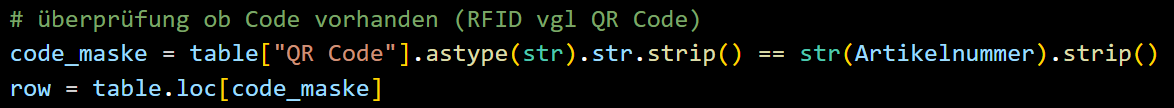
\includegraphics[width=0.9\textwidth]{Screenshots/Auftragsbasierte Auslagerung/CSV_Matching.png}
	\caption{Filterung der Materialdaten anhand der Artikelnummer}
	\label{fig:csv_Matching}
\end{figure}

In Abbildung \ref{fig:csv_Matching} ist der Abgleich der eingelesenen Daten mit den von der SPS bereitgestellten Werten dargestellt. Hierbei werden die Artikelnummern aus beiden Systemen miteinander verglichen.\\

Da die Daten aus unterschiedlichen Quellen stammen, wird zunächst eine Umwandlung in einen einheitlichen Datentyp durchgeführt. Dies erfolgt durch einen sogenannten \textit{String-Cast}, wodurch sichergestellt wird, dass die Vergleichsoperation korrekt durchgeführt werden kann.\\

Das Ergebnis dieses Vergleichs wird in einer logischen Maske (z.\,B. \texttt{code\_maske}) gespeichert. Diese Maske dient anschließend dazu, gezielt die entsprechende Zeile innerhalb der Tabelle auszuwählen.\\

Nach erfolgreicher Verarbeitung werden die aktualisierten Daten wieder in die CSV-Datei zurückgeschrieben. Dadurch bleibt die Datenbasis stets aktuell und reflektiert den Zustand des realen Lagersystems.\\
\begin{figure}[H]
	\centering
	\includegraphics[width=0.7\textwidth]{Screenshots/Auftragsbasierte Auslagerung/CSV_Update.png}
	\caption{Aktualisierung der Lagerplatzdaten in der CSV-Datei}
	\label{fig:csv_Update}
\end{figure}

Mithilfe der \texttt{.loc}-Funktion wird gezielt auf die zuvor gefilterten Einträge innerhalb der Tabelle zugegriffen. Dies ermöglicht eine direkte Aktualisierung der Lagerplatzdaten für das jeweilige Material.\\

Die neuen Werte, beispielsweise \texttt{Lagerplatz\_x} und \texttt{Lagerplatz\_y}, werden aus der SPS übernommen und in die entsprechenden Spalten der CSV-Datei eingetragen.\\

Nach der erfolgten Aktualisierung wird die Tabelle wieder in die CSV-Datei zurückgeschrieben. Dadurch bleibt die Datenbasis konsistent und spiegelt jederzeit den aktuellen Zustand des Lagersystems wider.
\subsubsection{Auslagerprozess innerhalb der Programmanwendung}

Für die Umsetzung des auftragsbasierten Auslagerprozesses wurde die Funktion \texttt{Auslagern} entwickelt. Diese übernimmt die Aufgabe, einen durch den Scanner erfassten Code auszuwerten und die entsprechenden Steuerinformationen für die Anlage zu generieren.\\

Zunächst wird die bestehende CSV-Datei eingelesen und anhand des übergebenen Codes gefiltert. Der Code dient dabei als eindeutige Identifikation des Materials. Wird ein entsprechender Datensatz gefunden, werden die zugehörigen Lagerplatzinformationen extrahiert\ref{fig:csv_Zuordnung}.\\
\begin{figure}[H]
	\centering
	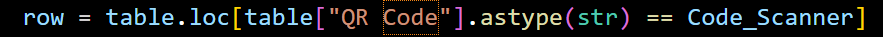
\includegraphics[width=0.7\textwidth]{Screenshots/Auftragsbasierte Auslagerung/CSV_Zuordnung.png}
	\caption{Zuordnung eines gescannten Codes zu einem Materialdatensatz}
	\label{fig:csv_Zuordnung}
\end{figure}
Im Anschluss erfolgt eine Überprüfung, ob für das ausgewählte Material gültige Lagerplatzdaten vorliegen. Ist dies nicht der Fall, wird der Prozess abgebrochen, um fehlerhafte Zustände zu vermeiden.\\

Sind gültige Daten vorhanden, werden diese für die weitere Nutzung aufbereitet und an die \textbf{SPS} übergeben. Hierfür wird eine separate Funktion verwendet, welche die Daten in das entsprechende Format überführt und in die relevanten Speicherbereiche der Steuerung schreibt\ref{fig:Daten_an_SPS}.\\
\begin{figure}[H]
	\centering
	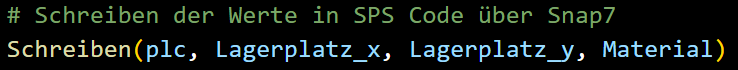
\includegraphics[width=0.7\textwidth]{Screenshots/Auftragsbasierte Auslagerung/Python_SPS.png}
	\caption{Übergabe der berechneten Daten an die SPS}
	\label{fig:Daten_an_SPS}
\end{figure}
Zusätzlich wird jede Durchführung eines Ein- oder Auslagerprozesses protokolliert. Diese Historie ermöglicht eine Nachvollziehbarkeit der durchgeführten Aktionen und dient der Analyse des Systemverhaltens.

\subsubsection{Einlesen von Daten aus der SPS}

Zur Kommunikation mit der Steuerung wurde eine Funktion \texttt{Einlesen} implementiert. Diese greift über die Snap7-Schnittstelle auf definierte Datenbausteine der \textbf{SPS} zu und liest die dort abgelegten Werte aus.\\

Dabei werden insbesondere Koordinatenwerte sowie Artikelinformationen in Python-Variablen überführt und für weitere Verarbeitungsschritte bereitgestellt.

\subsubsection{Übertragung von Daten an die SPS}

Für die Übergabe von Steuerinformationen an die Anlage wurde die Funktion \texttt{Schreiben} realisiert. Diese transformiert die in Python vorliegenden Daten in das benötigte Byteformat und überträgt diese in die entsprechenden Datenbereiche der \textbf{SPS}.\\

Durch das Setzen dieser Werte wird der eigentliche Auslagerprozess innerhalb der Steuerung ausgelöst.

\subsubsection{Erfassung von Scannerdaten}

Die Erfassung der Auftragsdaten erfolgt über einen seriell angebundenen Scanner. Hierfür wurde eine Funktion zur kontinuierlichen Datenerfassung implementiert. Die empfangenen Daten werden als Zeichenkette eingelesen und anschließend bereinigt.\\
\begin{figure}[H]
	\centering
	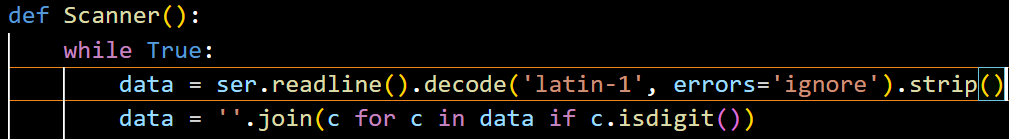
\includegraphics[width=0.8\textwidth]{Screenshots/Auftragsbasierte Auslagerung/Scanner.png}
	\caption{Einlesen und Bereinigung der Scannerdaten}
	\label{fig:Scan_Einlesen}
\end{figure}

In Abbildung \ref{fig:Scan_Einlesen} ist der Prozess des Einlesens und der anschließenden Verarbeitung der Scannerdaten dargestellt. Die Daten werden über eine serielle Schnittstelle empfangen und zunächst als Rohdaten eingelesen.\\

Da die übertragenen Daten neben der eigentlichen Information zusätzliche Zeichen enthalten können, erfolgt im nächsten Schritt eine Bereinigung der Daten.\\
Hierbei werden ausschließlich numerische Zeichen extrahiert, sodass ein eindeutiger Code zur weiteren Verarbeitung entsteht.

Durch diese Verarbeitung wird sichergestellt, dass nur gültige und verwertbare Daten im System verwendet werden. Der bereinigte Code dient anschließend als Grundlage für die Identifikation des entsprechenden Materials innerhalb der Datenbank und wird weiter im Auslagerprozess verwendet.\\

Die kontinuierliche Überwachung der Schnittstelle stellt sicher, dass eingehende Daten unmittelbar verarbeitet werden können. Eine zukünftige Erweiterung des Systems sieht hierbei eine Parallelisierung der Datenverarbeitung vor.\\

Im folgenden Kapitel werden die notwendigen Anpassungen im SPS Programm erläutert um eine erfolgreicvhe Auftragssteurung zu gewährleisten.